\documentclass[letterpaper, reqno,11pt]{article}
\usepackage[margin=1.0in]{geometry}
\usepackage{color,latexsym,amsmath,amssymb,graphicx,float,listings,tikz}
\usepackage{hyperref}

\hypersetup{
colorlinks=true,
linkcolor=magenta,
filecolor=magenta,
urlcolor=cyan,
}

\graphicspath{ {images/} }

\begin{document}
\pagenumbering{arabic}

\begin{titlepage}
\newgeometry{margin=3cm}
\centering

\vspace*{\stretch{2}}

\Large ELEC 302 Lab 2 Report

\vspace{\stretch{1}}

\normalsize Bistable and Monostable Multivibrators

\vspace{\stretch{0.5}}

\begin{tabular}{ll}
Name & Xander Naumenko \\[2ex]
Student Number  & 38198354 \\[2ex]
Lab Group            & L2C \\[2ex]
Experiment Date            & 2023-03-04 \\[2ex]
Partner's Name &  Brian Sun
\end{tabular}

\vspace{\stretch{3}}


\vspace{\stretch{2}}
\end{titlepage}

{\medskip\noindent\bf Question 1.1.} Using superposition, we have that:
\[
v_{+}= \frac{R_2}{R_1+R_2}v_{in}= \frac{R_1}{R_1+R_2}v_{out}
.\]
To trigger $v_0$ from $L_+$ to $L_-$, we start with $v_+>0$, so $v_0=L_+$. At the transition $v_+=0$, so we can solve for $v_{in}$:
\[
V_{TL}=-L_+ \frac{R_1}{R_2}
.\]
Repeating this same logic for the other direction, we get:
\[
V_{TH}= -L_- \frac{R_1}{R_2}
.\]

{\medskip\noindent\bf Question 1.2.} Solving the equations derived in part 1:

\[
\frac{R_2}{R_1}=\frac{L_+}{3}=\frac{14}{3}\approx 4.67
.\]
Thus as  good approxmation we used a $4.7\text{k}\Omega$ and a $1\text{k}\Omega$ resistor for a ratio of $4.7$.

{\medskip\noindent\bf Question 1.3.} No questions for this part.

{\medskip\noindent\bf Question 1.4.} See figures \ref{fig:1-4} and \ref{fig:1-5} for the time and XY plots respectively. Experimentally, by lowering $V_{in}$ until the trigger points were no longer seen, it was at around $V_{in}=6.5$V that they stopped appearing. If the op-amp was ideal then in theory the we would only need $V_{pp}=V_{TH}+V_{TL}=2\cdot 3=6$V. Probably the most likely cause of this discrepancy is the saturation voltage of the op-amp not being exactly $14V$ for a power supply of $15$, as this values was assumed when calculating the required voltage ratio.

\begin{figure}[htpb]
    \centering
    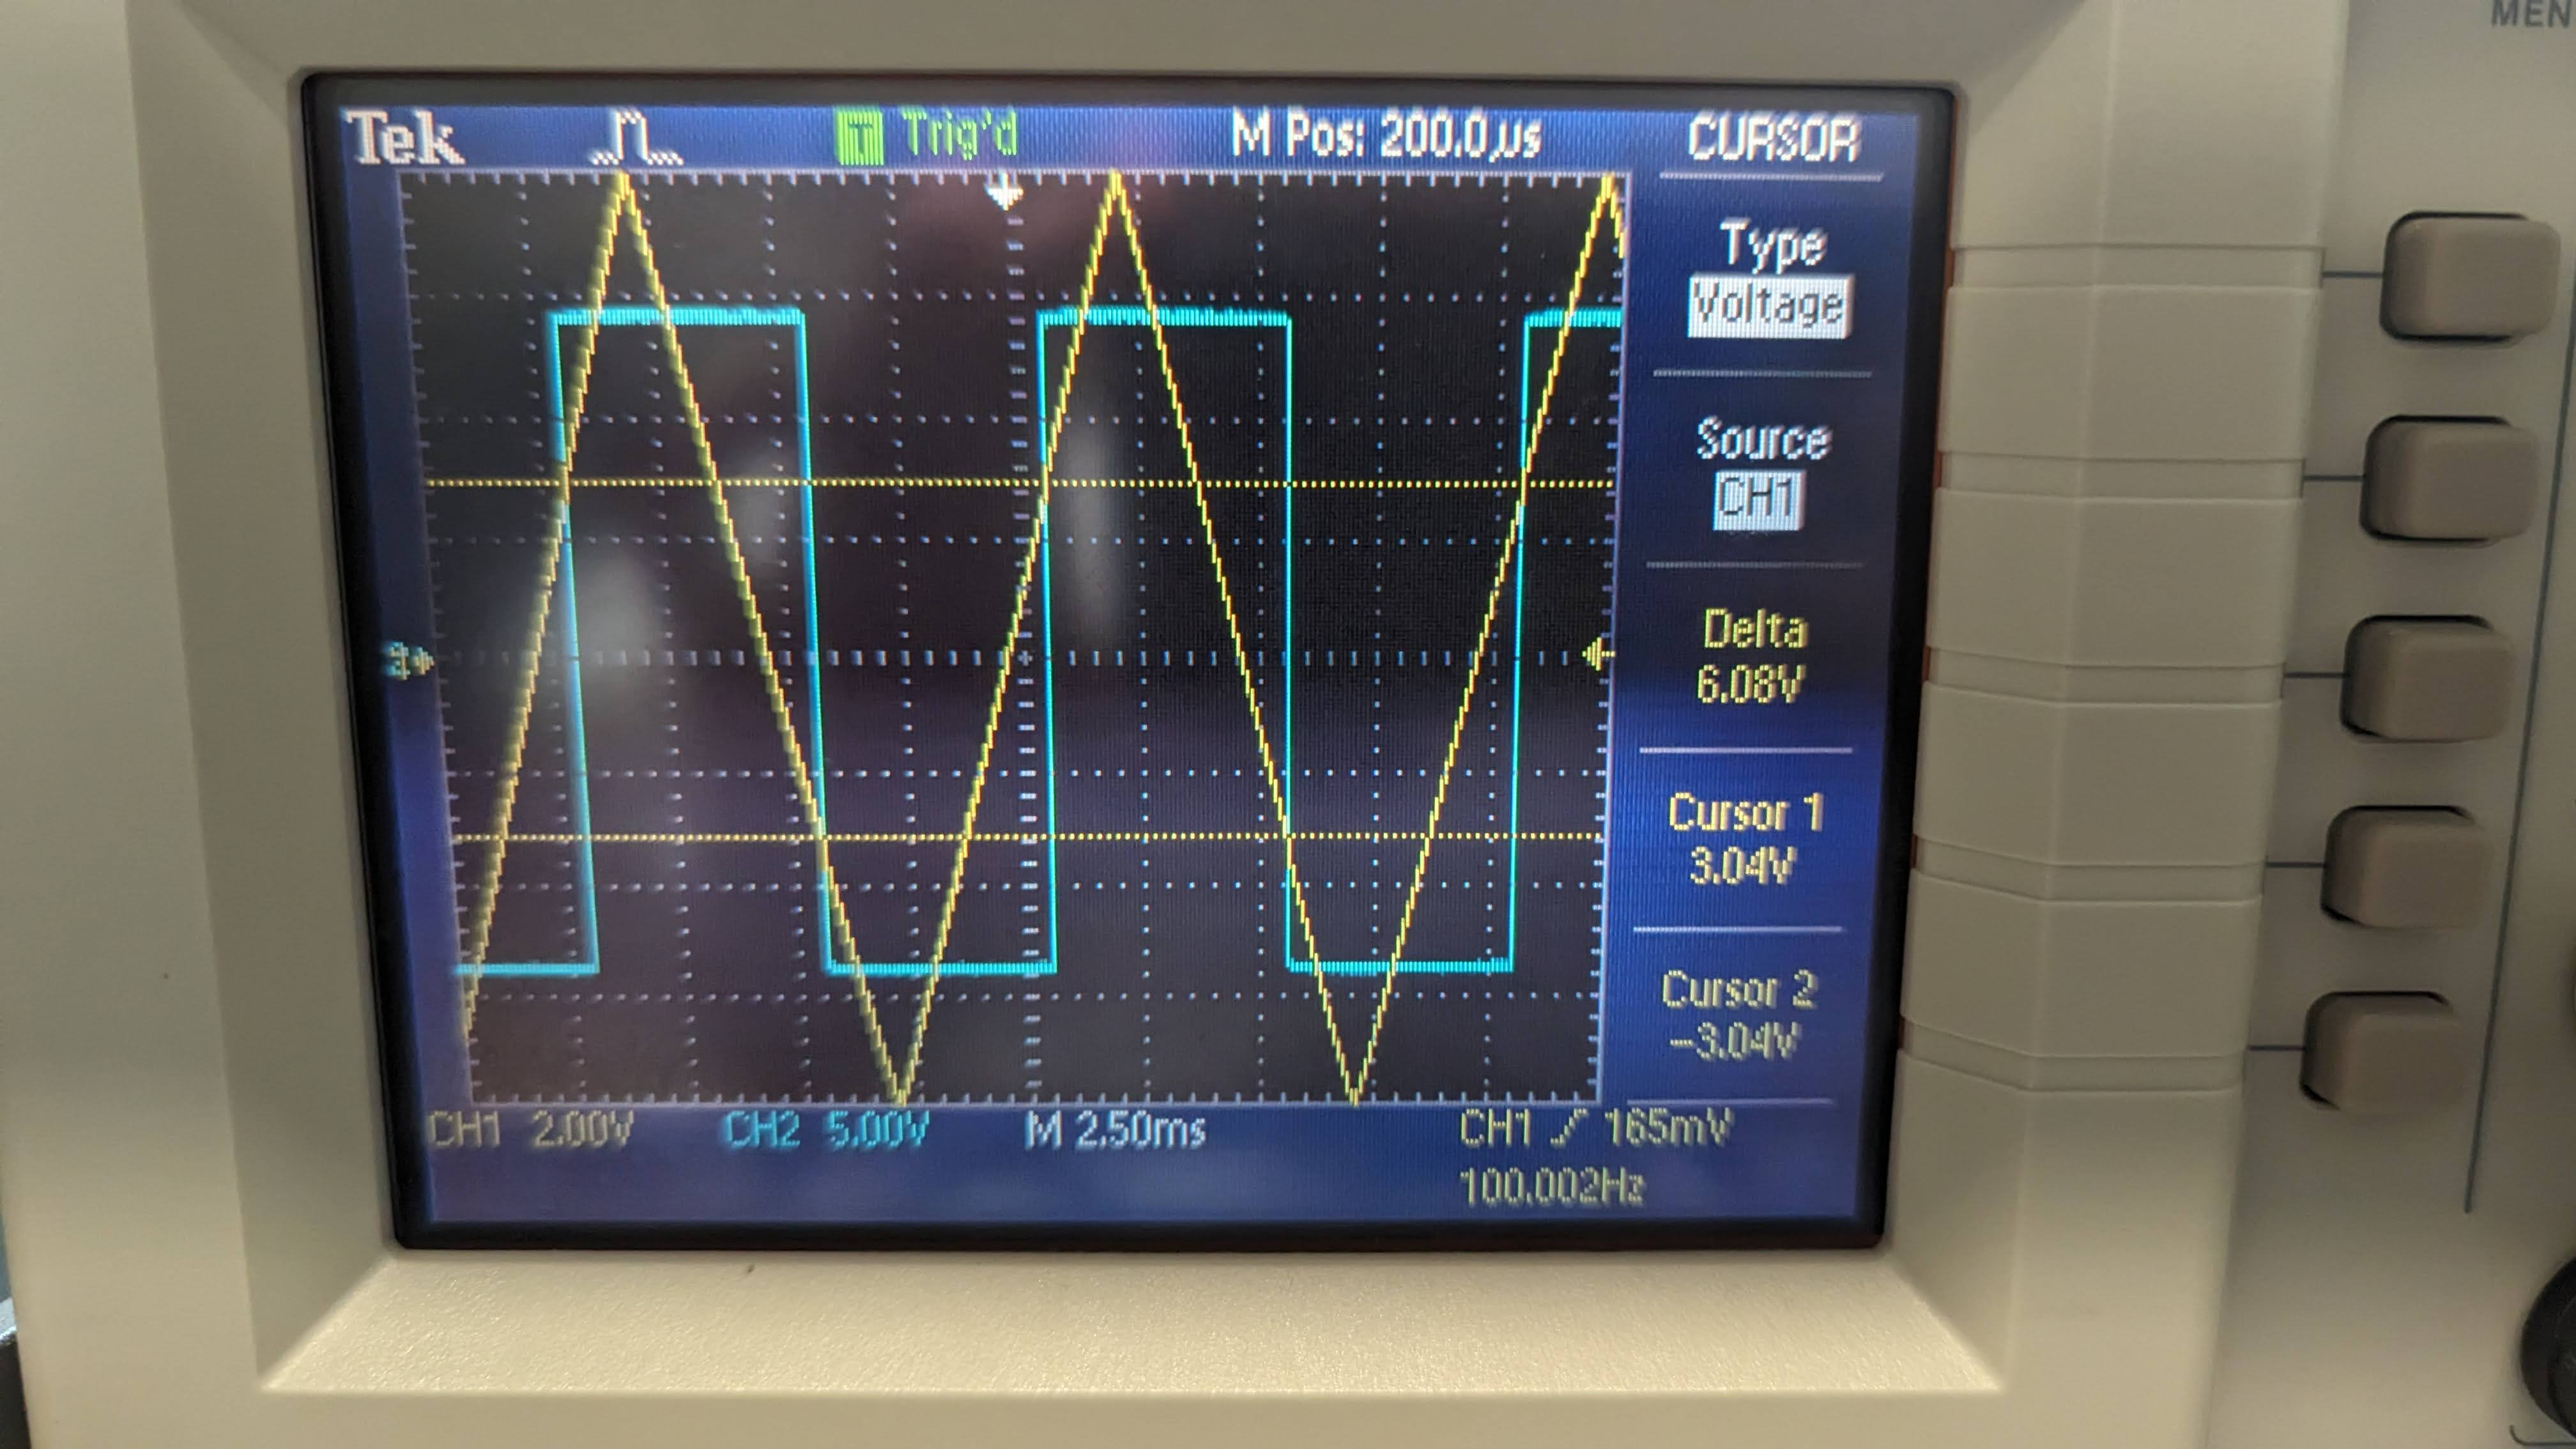
\includegraphics[width=0.8\textwidth]{1-4}
    \caption{Time plot of Schmitt trigger. Yellow is input triangle wave, blue is output voltage of Schmitt trigger. As seen by the cursors the crossover voltages are approximately $3$V, as they were designed to be.}
    \label{fig:1-4}
\end{figure}

\begin{figure}[htpb]
    \centering
    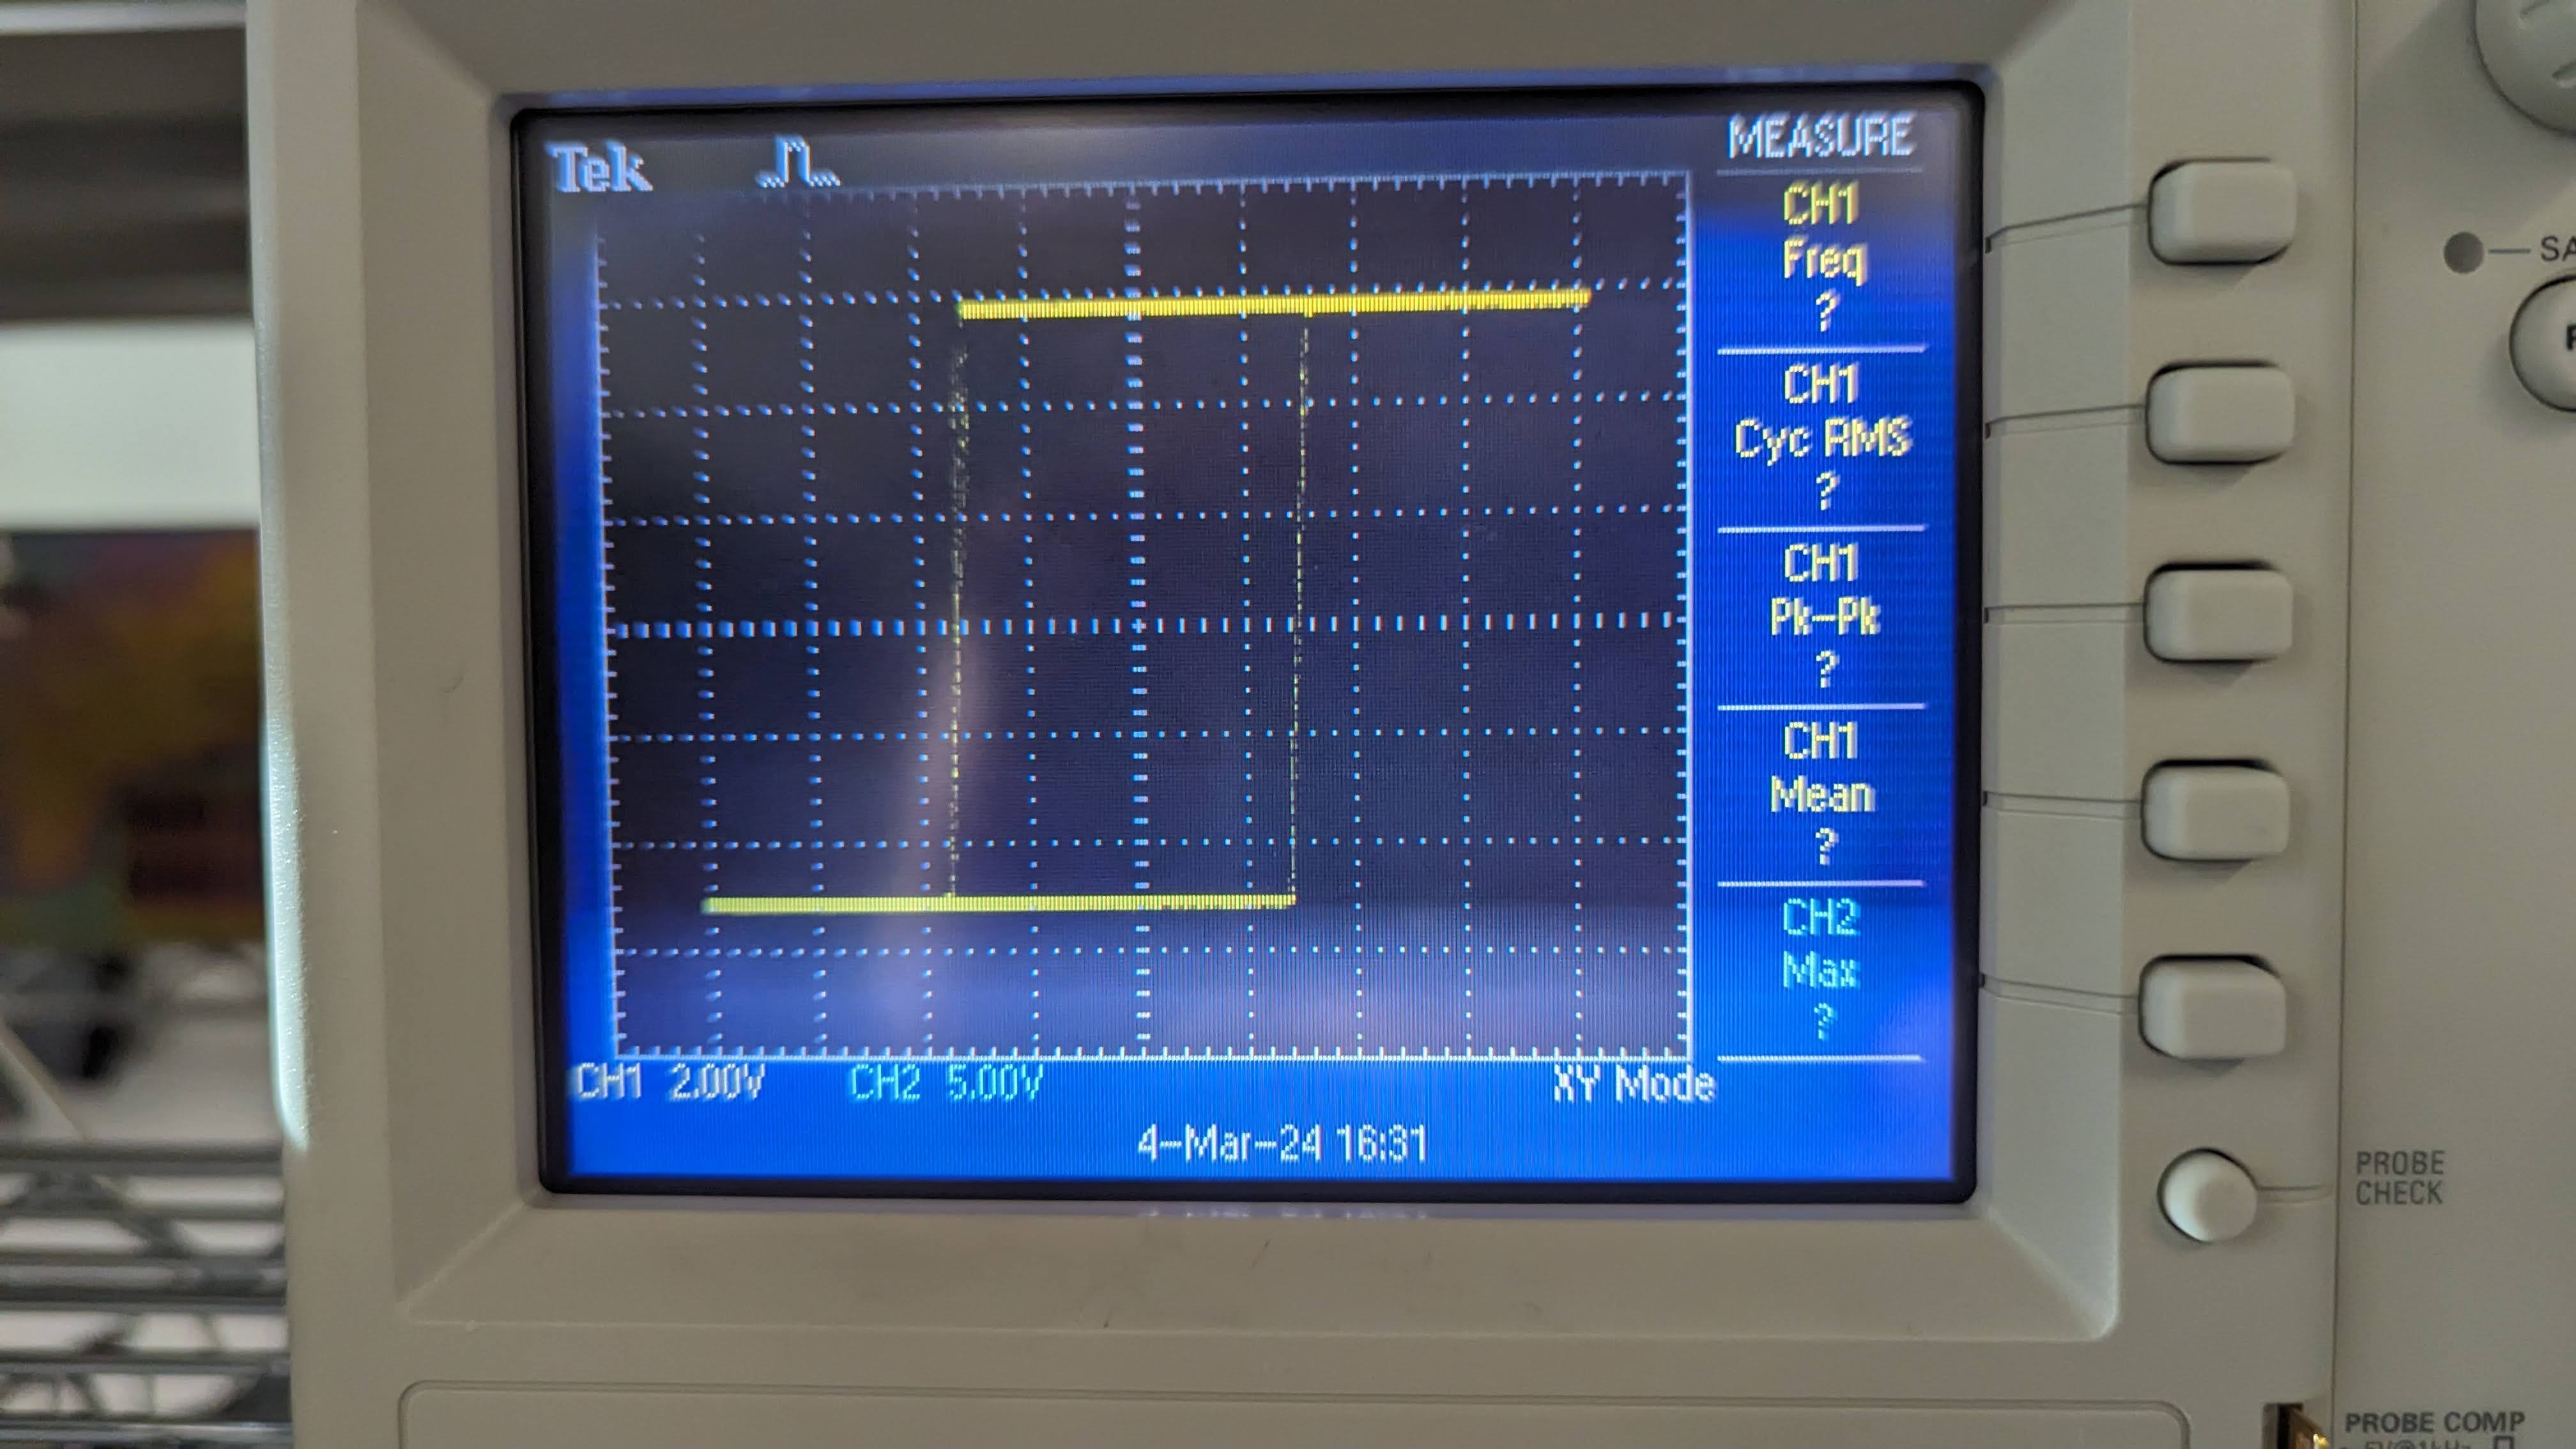
\includegraphics[width=0.8\textwidth]{1-5}
    \caption{DC transfer characteristic of the Schmitt trigger. As expected, the transition between levels is almost instantaneous, hence the thin vertical lines.}
    \label{fig:1-5}
\end{figure}

{\medskip\noindent\bf Question 1.5.} See figure \ref{fig:1-5} for the measured transfer characteristic. See table \ref{tab:1-5} for a table of the required values. $V_{t1}$ and $V_{t2}$ were both very close to the theoretical value, $\pm 0.04$ is definitely within the experimental uncertainty of positioning the cursors on the oscilloscope. $L_+$ and $L_-$ were slightly higher in magnitude than the $14$V that was expected. The most likely possibility for this is the variation in the op-amp itself, as the saturation voltage for a given input may not be consistent between ICs. It could also be that the input voltage was set slightly high, as the dial to set it is rather sensitive and they weren't double checked later in the lab.

\begin{table}[htpb]
    \centering
    \caption{Measured values for question 1.5.}
    \label{tab:1-5}
    \begin{tabular}{|c|c|}
        \hline
        Quantity & Value\\
        \hline 
        $L_{+}$&14.2V\\
        $L_-$&-14.1V\\
        $V_{t1}$&3.04V\\
        $V_{t2}$&-3.04V\\
        \hline
    \end{tabular}
\end{table}

{\medskip\noindent\bf Question 2.1.} The required values for everything except $V_{ref}$ was given to us, see figure \ref{fig:2-1}. See \ref{tab:2-1} for the values in tabular form. From the prelab, $T=RC\text{ln} \frac{V_+-V_-}{V_{ref}}$, which we can solve to give $-V_{ref}=1.4$V. This was achieve by using a potentiometer between $-15$V and ground and experimentally adjusting it until a voltage of $-1.4$V was read on the digital multimeter. Note that originally the built in potentiometer on the breadboard was used, but because it had low impedance it was subject to variations of voltage when load was applied in later parts. Therefore an external potentiometer with $1$k$\Omega$-10k$\Omega$ was used instead.

\begin{figure}[htpb]
    \centering
    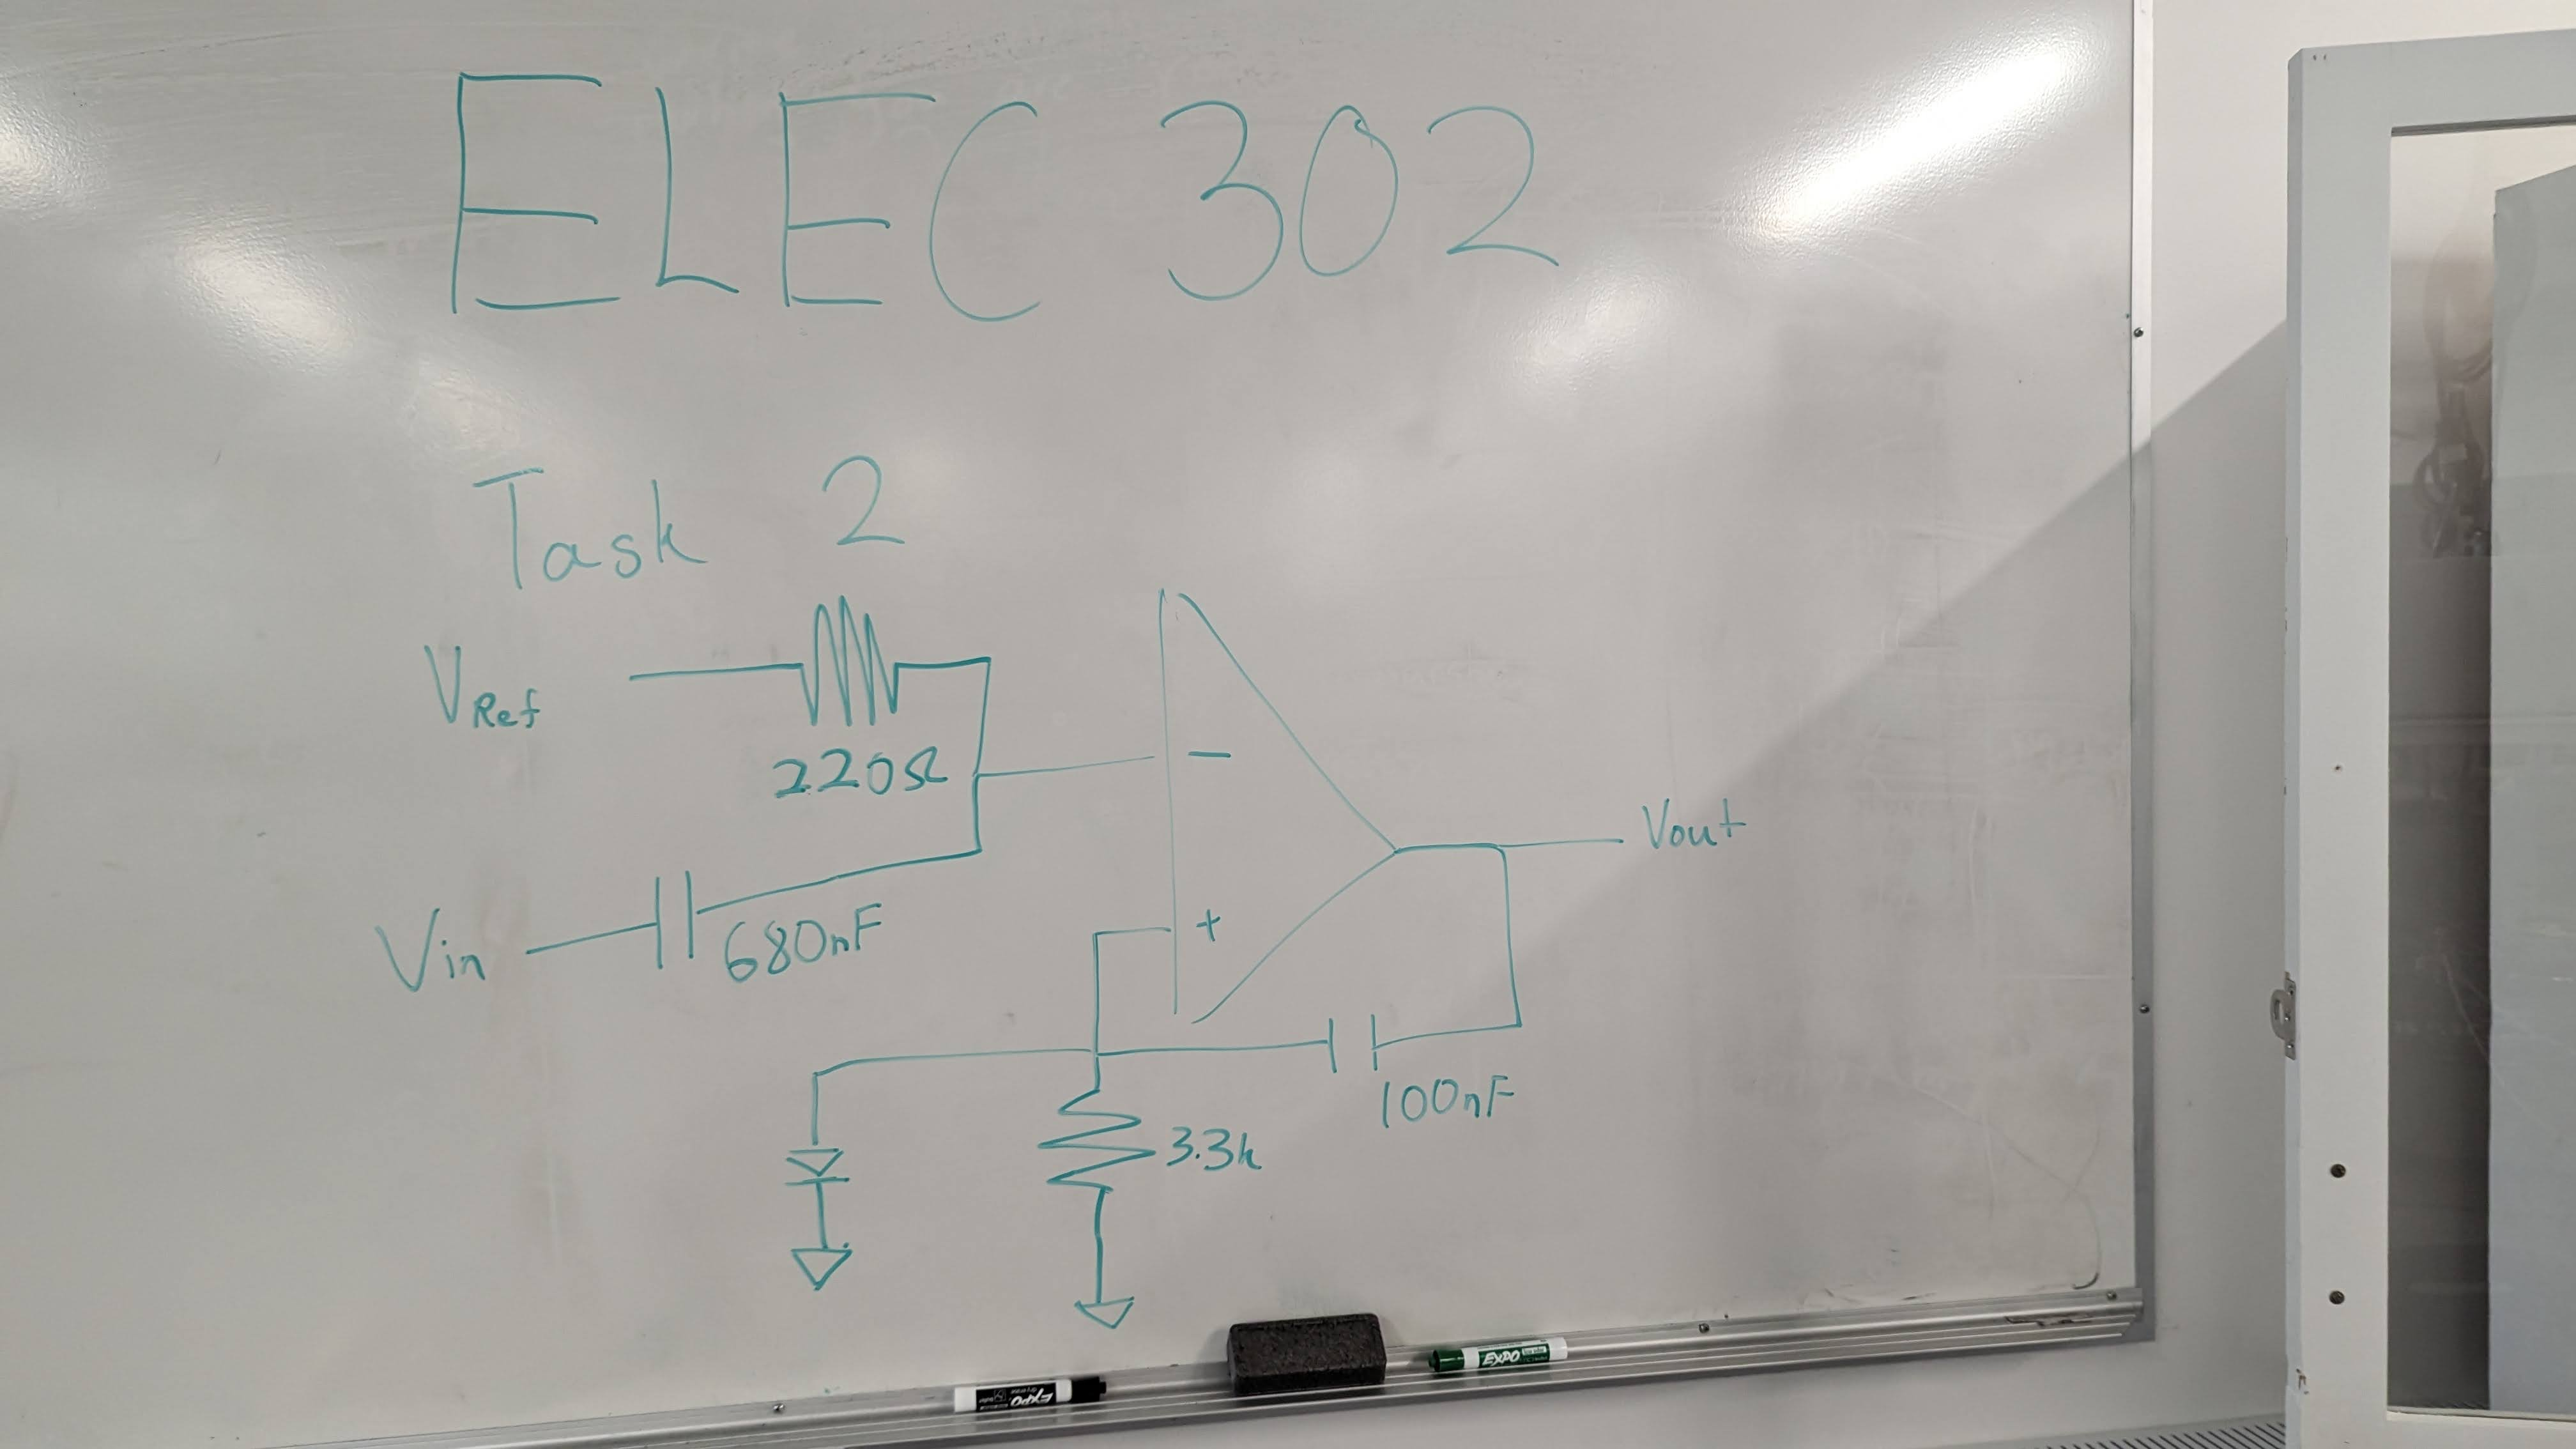
\includegraphics[width=0.8\textwidth]{2-1}
    \caption{Circuit diagram with values for question 2.1.}
    \label{fig:2-1}
\end{figure}

\begin{table}[htpb]
    \centering
    \caption{Parameters for question 2-1.}
    \label{tab:1-5}
    \begin{tabular}{|c|c|}
        \hline
        Quantity & Value\\
        \hline 
        $R_1$&220$\Omega$\\
        $C_1$&680nF\\
        $R_2$&$3300\Omega$\\
        $C_2$&100nF\\
        $-V_{ref}$&1.4V\\
        \hline
    \end{tabular}
\end{table}

{\medskip\noindent\bf Question 2.2.} See figure \ref{fig:2-2} for the plots. The width of the pulse was $1.32$ms, which is considerably higher than the predicted $1$ms. Experimentally, by changing $-V_{ref}$, a pulse width of $1$ms was obtained when $V_{ref}=-2.75$.

\begin{figure}[htpb]
    \centering
    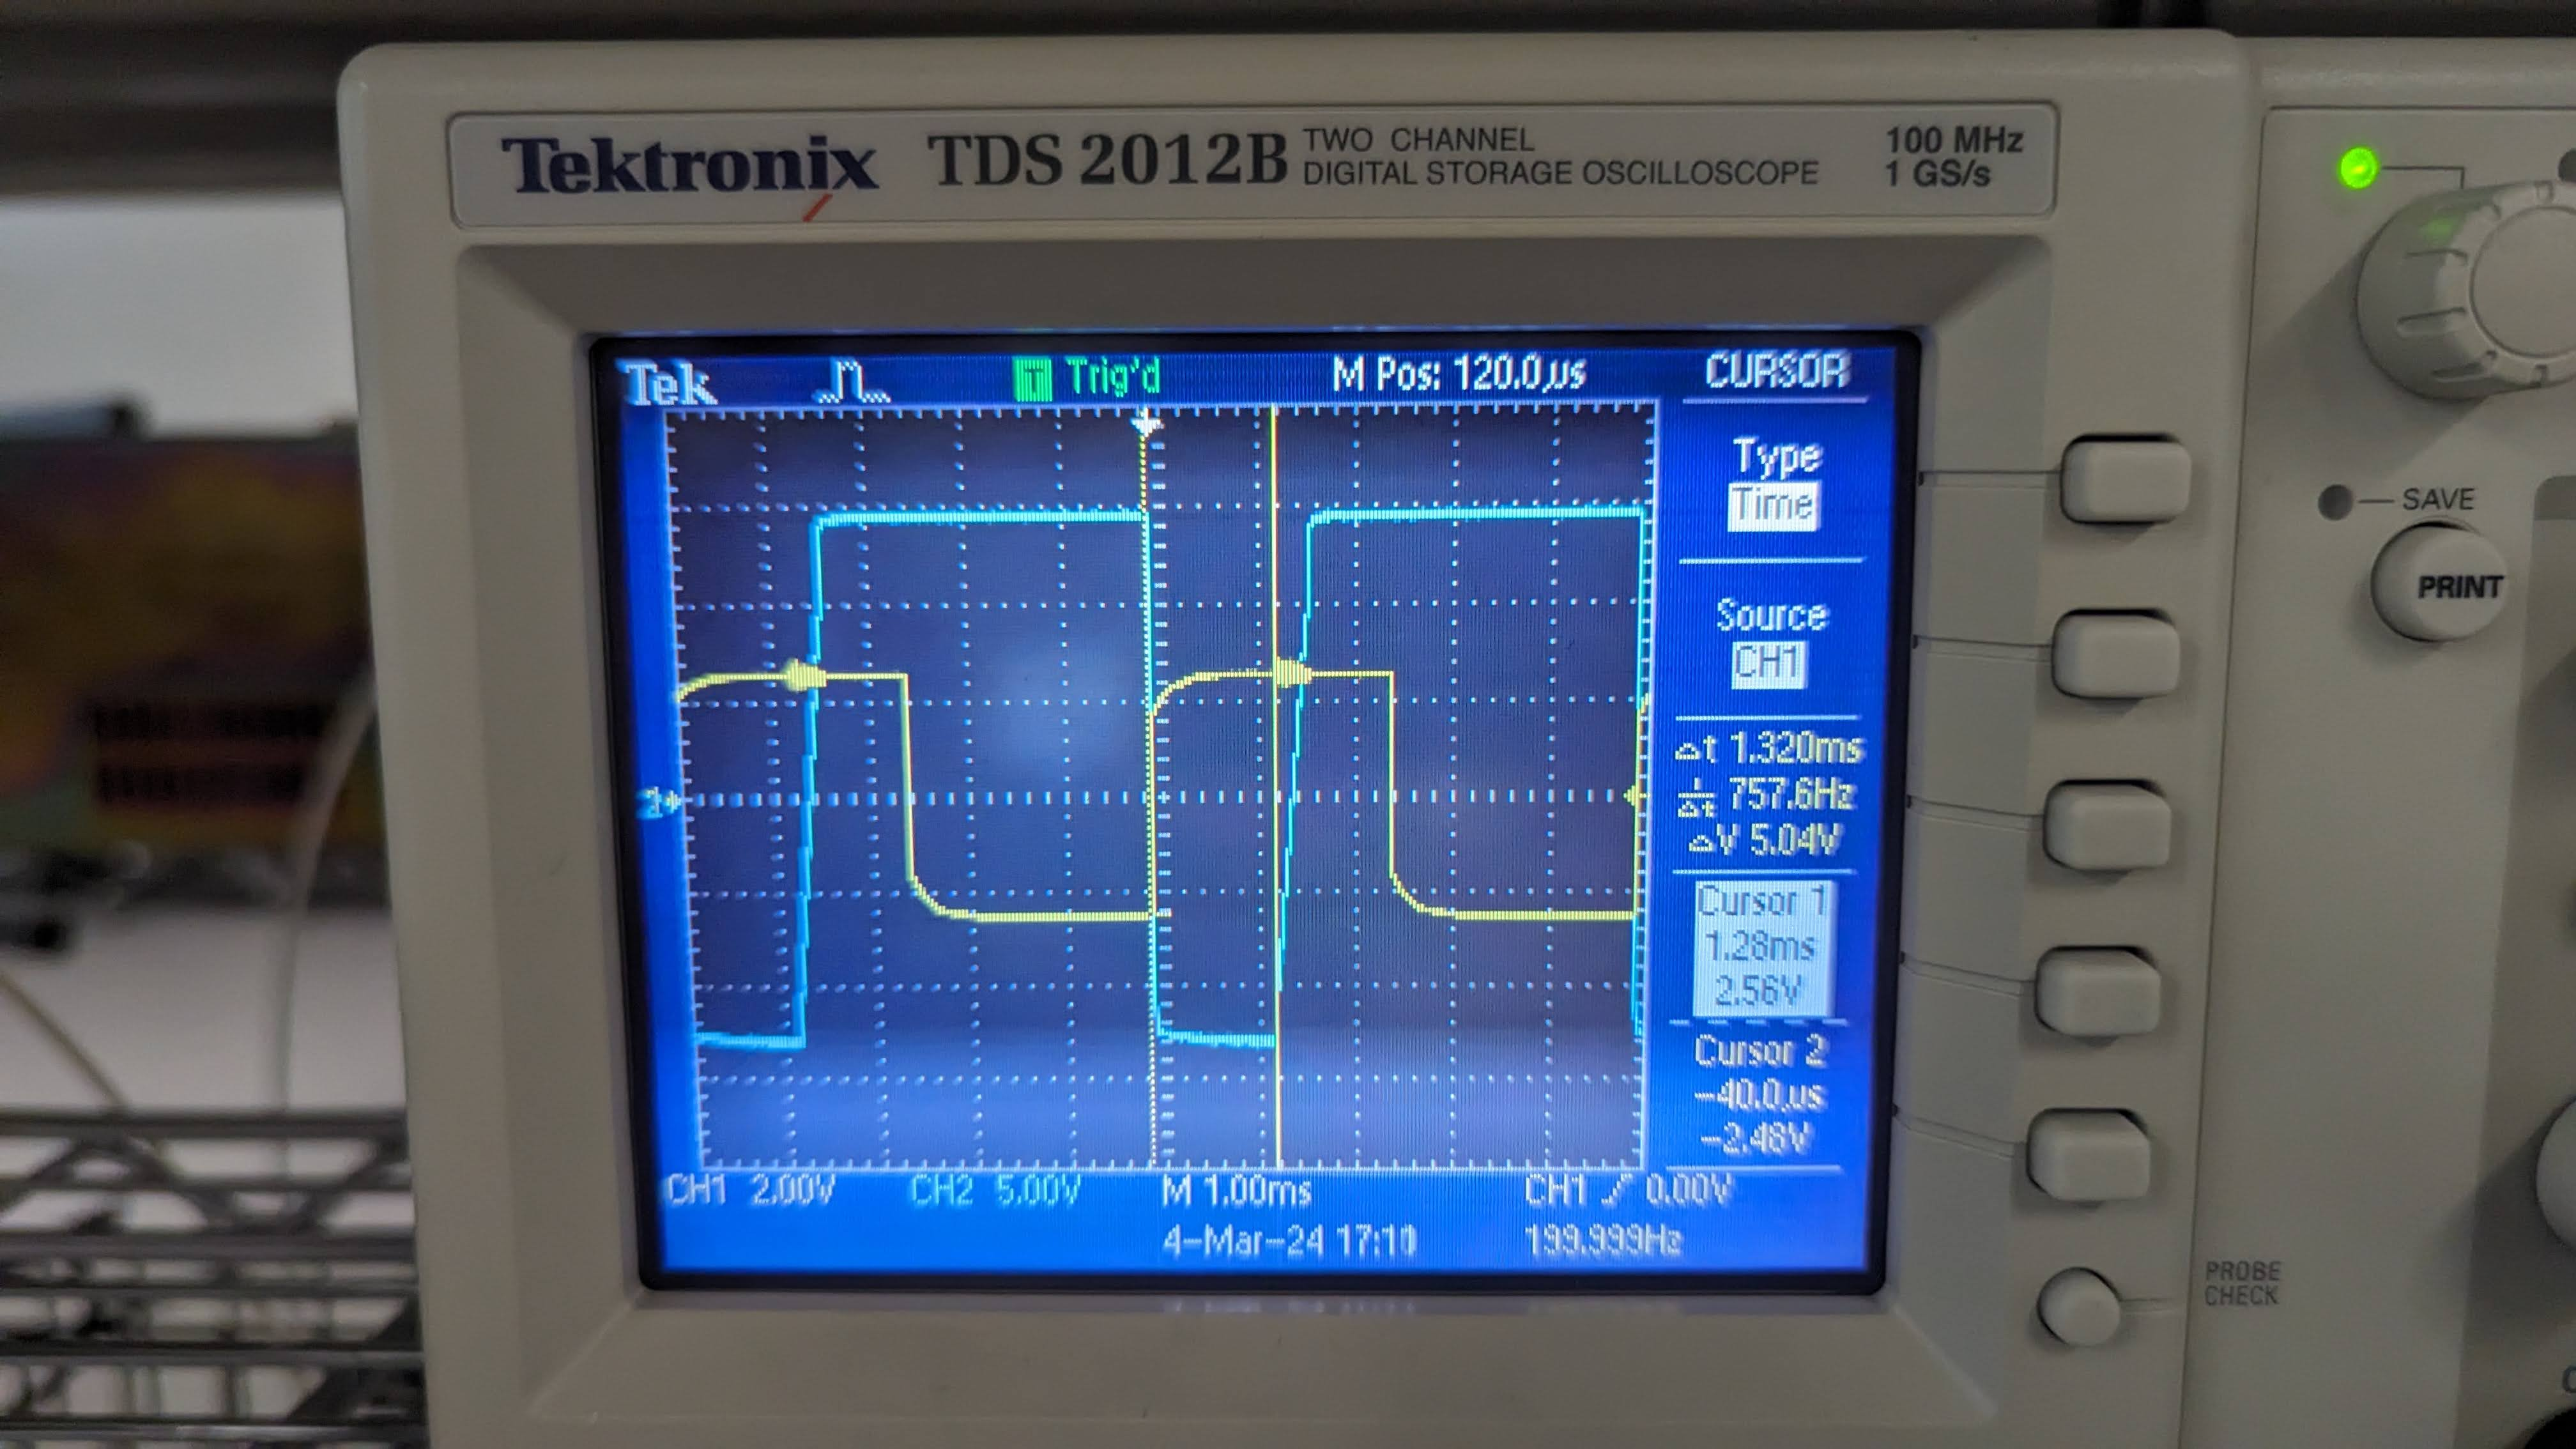
\includegraphics[width=0.45\textwidth]{2-2-Vout}
    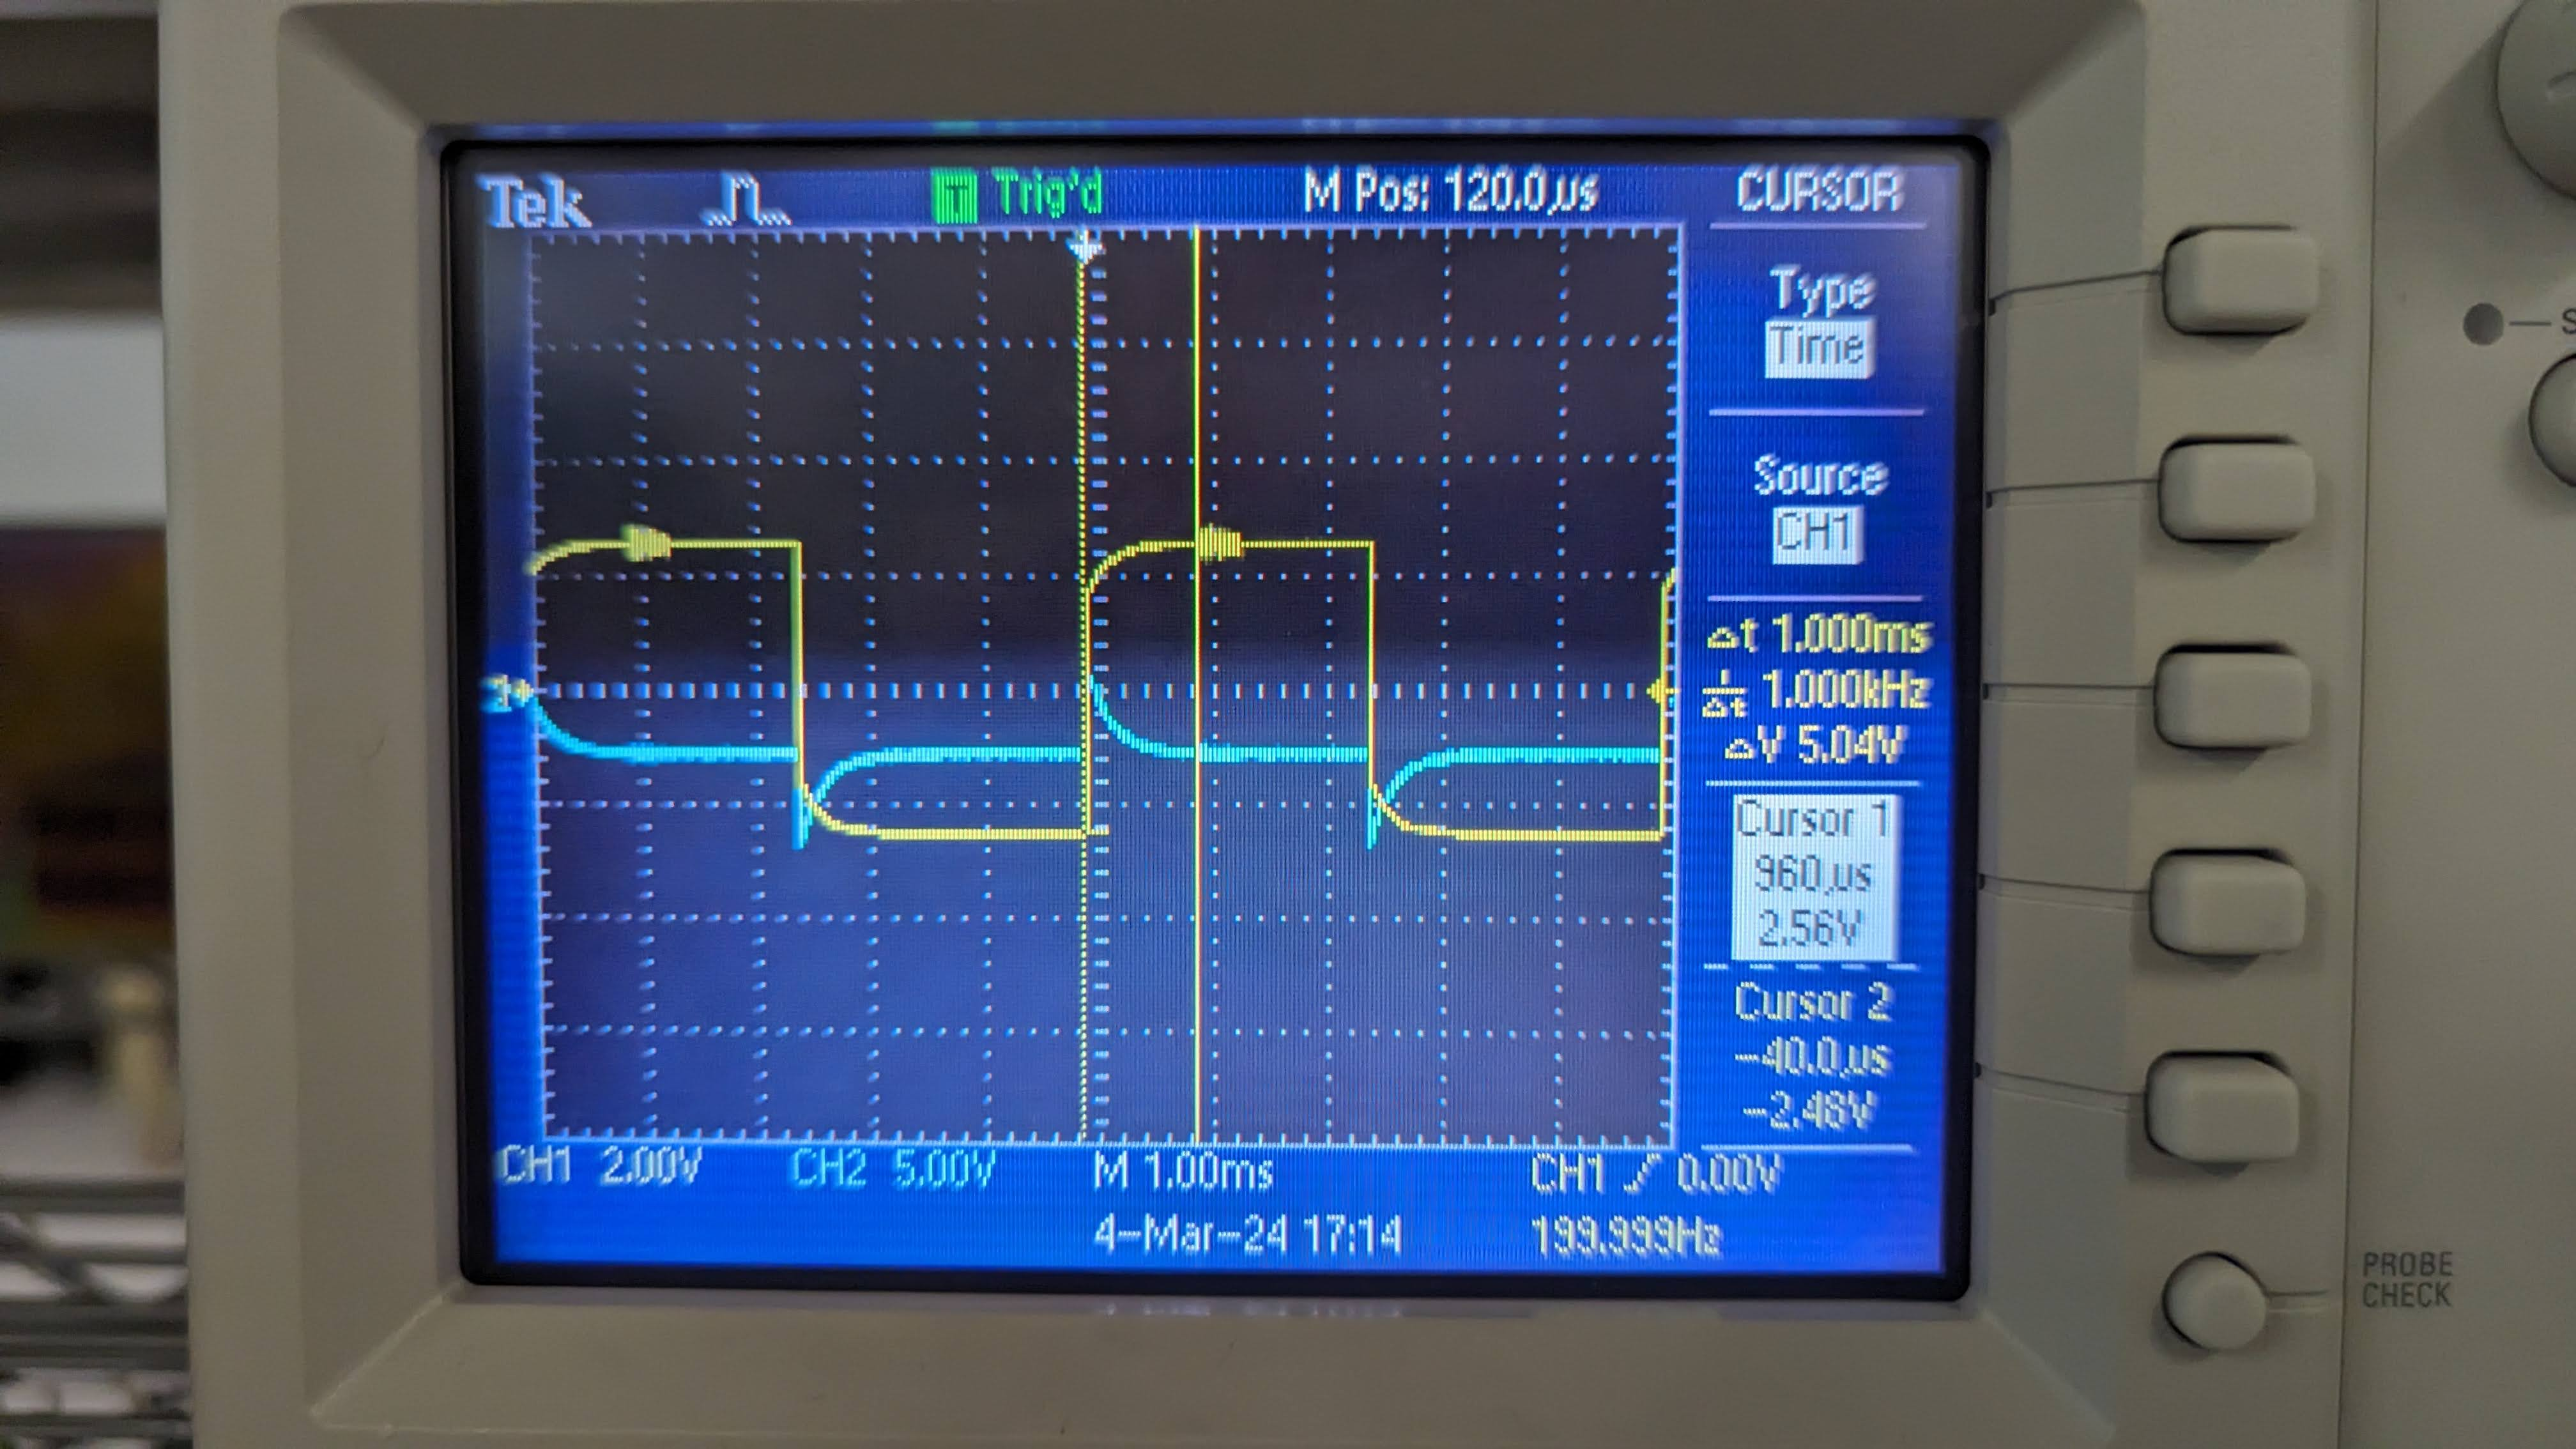
\includegraphics[width=0.45\textwidth]{2-2-A}
    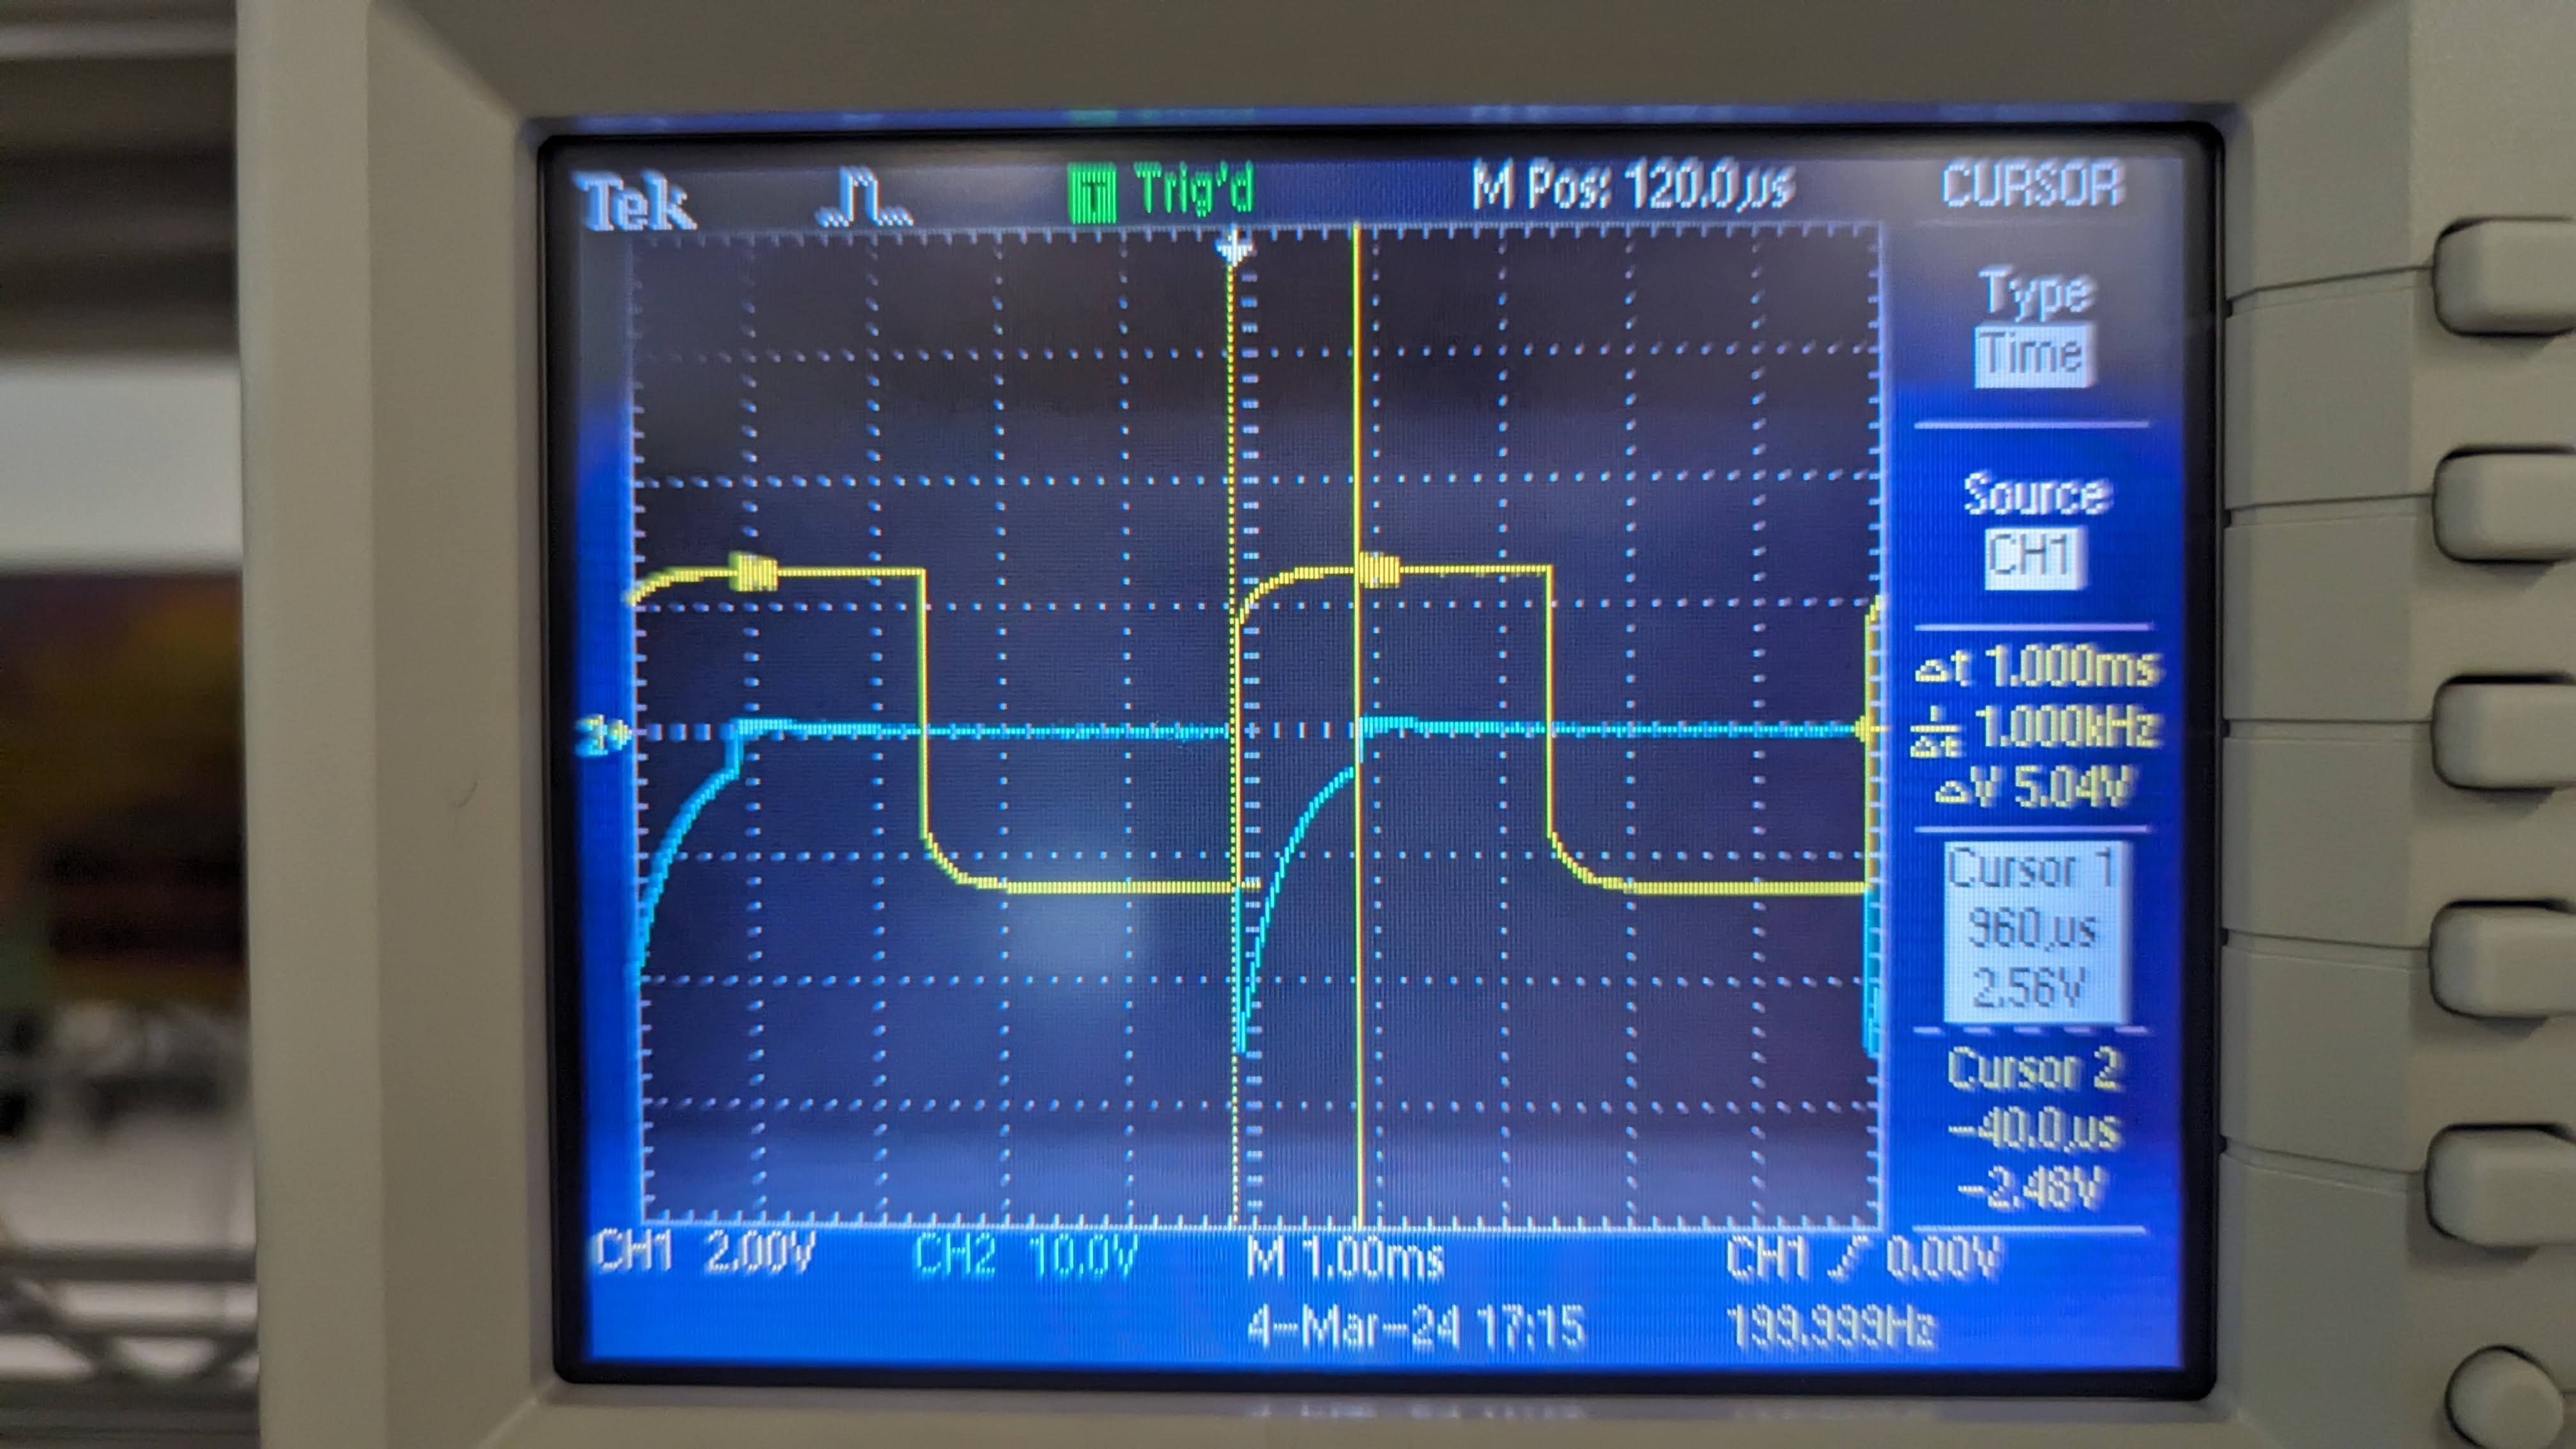
\includegraphics[width=0.45\textwidth]{2-2-B}
    \caption{Plots for question 2.2. In order these show $V_{out}$, $V_A$ and $V_B$ respectively in blue, with $V_{in}$ in yellow on all of them. At $B$ the voltage is as expected, with $C_1$ charging and discharging every time $V_{in}$ switches sign. $A$ is also mostly expected with the instantaneous drop then the charging of $C_2$. The sloped line of $V_{in}$ on the way up was not expected by me, and was initially confusing. I think the most likely reason for it is the finite gain of the op-amp, as although in theory it is infinite, for a period when $C_2$ is almost discharged, $V_+-V_-$ is nonzero but very small, which means that the switch from $L_-$ to $L_+$ is non instantaneous.}
    \label{fig:2-2}
\end{figure}

{\medskip\noindent\bf Question 2.3.} The observed pulse of $1.32$ms was considerably off from the predicted pulse with of $1$ms. There are a few possible factors for the discrepancy. Firstly, the error in the components could be quite large. Uncertainty for capacitors often goes as high as $\pm 20\%$, so it's possible that this is at fault. After talking with other teams during the lab most others also had a pulse width greater than 1ms, and while there was significant variance this likely indicates there's also a systematic effect behind the wider pulse. One possible such systematic effect is that the saturation voltage of the op-amp isn't exactly $14$V, as in part 1 we saw that it wasn't exact.

{\medskip\noindent\bf Question 2.4.} See figure \ref{fig:2-4}. The resulting pulse width is $500$ms. This can be explained by the fact that the pulse is being ``squished'' when the input waveform's period is less than the normal pulse width. All the analysis in the prelab assumed that once $V_{in}$ goes from low to high, the system has time to settle before $V_{in}$ changes again. However in this case $V_{in}$ goes low again before $C_2$ has a chance to fully discharge, which causes $V_- <V_+$ so $V_{out}$ immediately goes high again. The result is that for $f>500$Hz, $V_{out}$ acts as an inverter of the given wave (timing wise at least, it's magnitude remains $L_-$ to $L_+$). 

\begin{figure}[htpb]
    \centering
    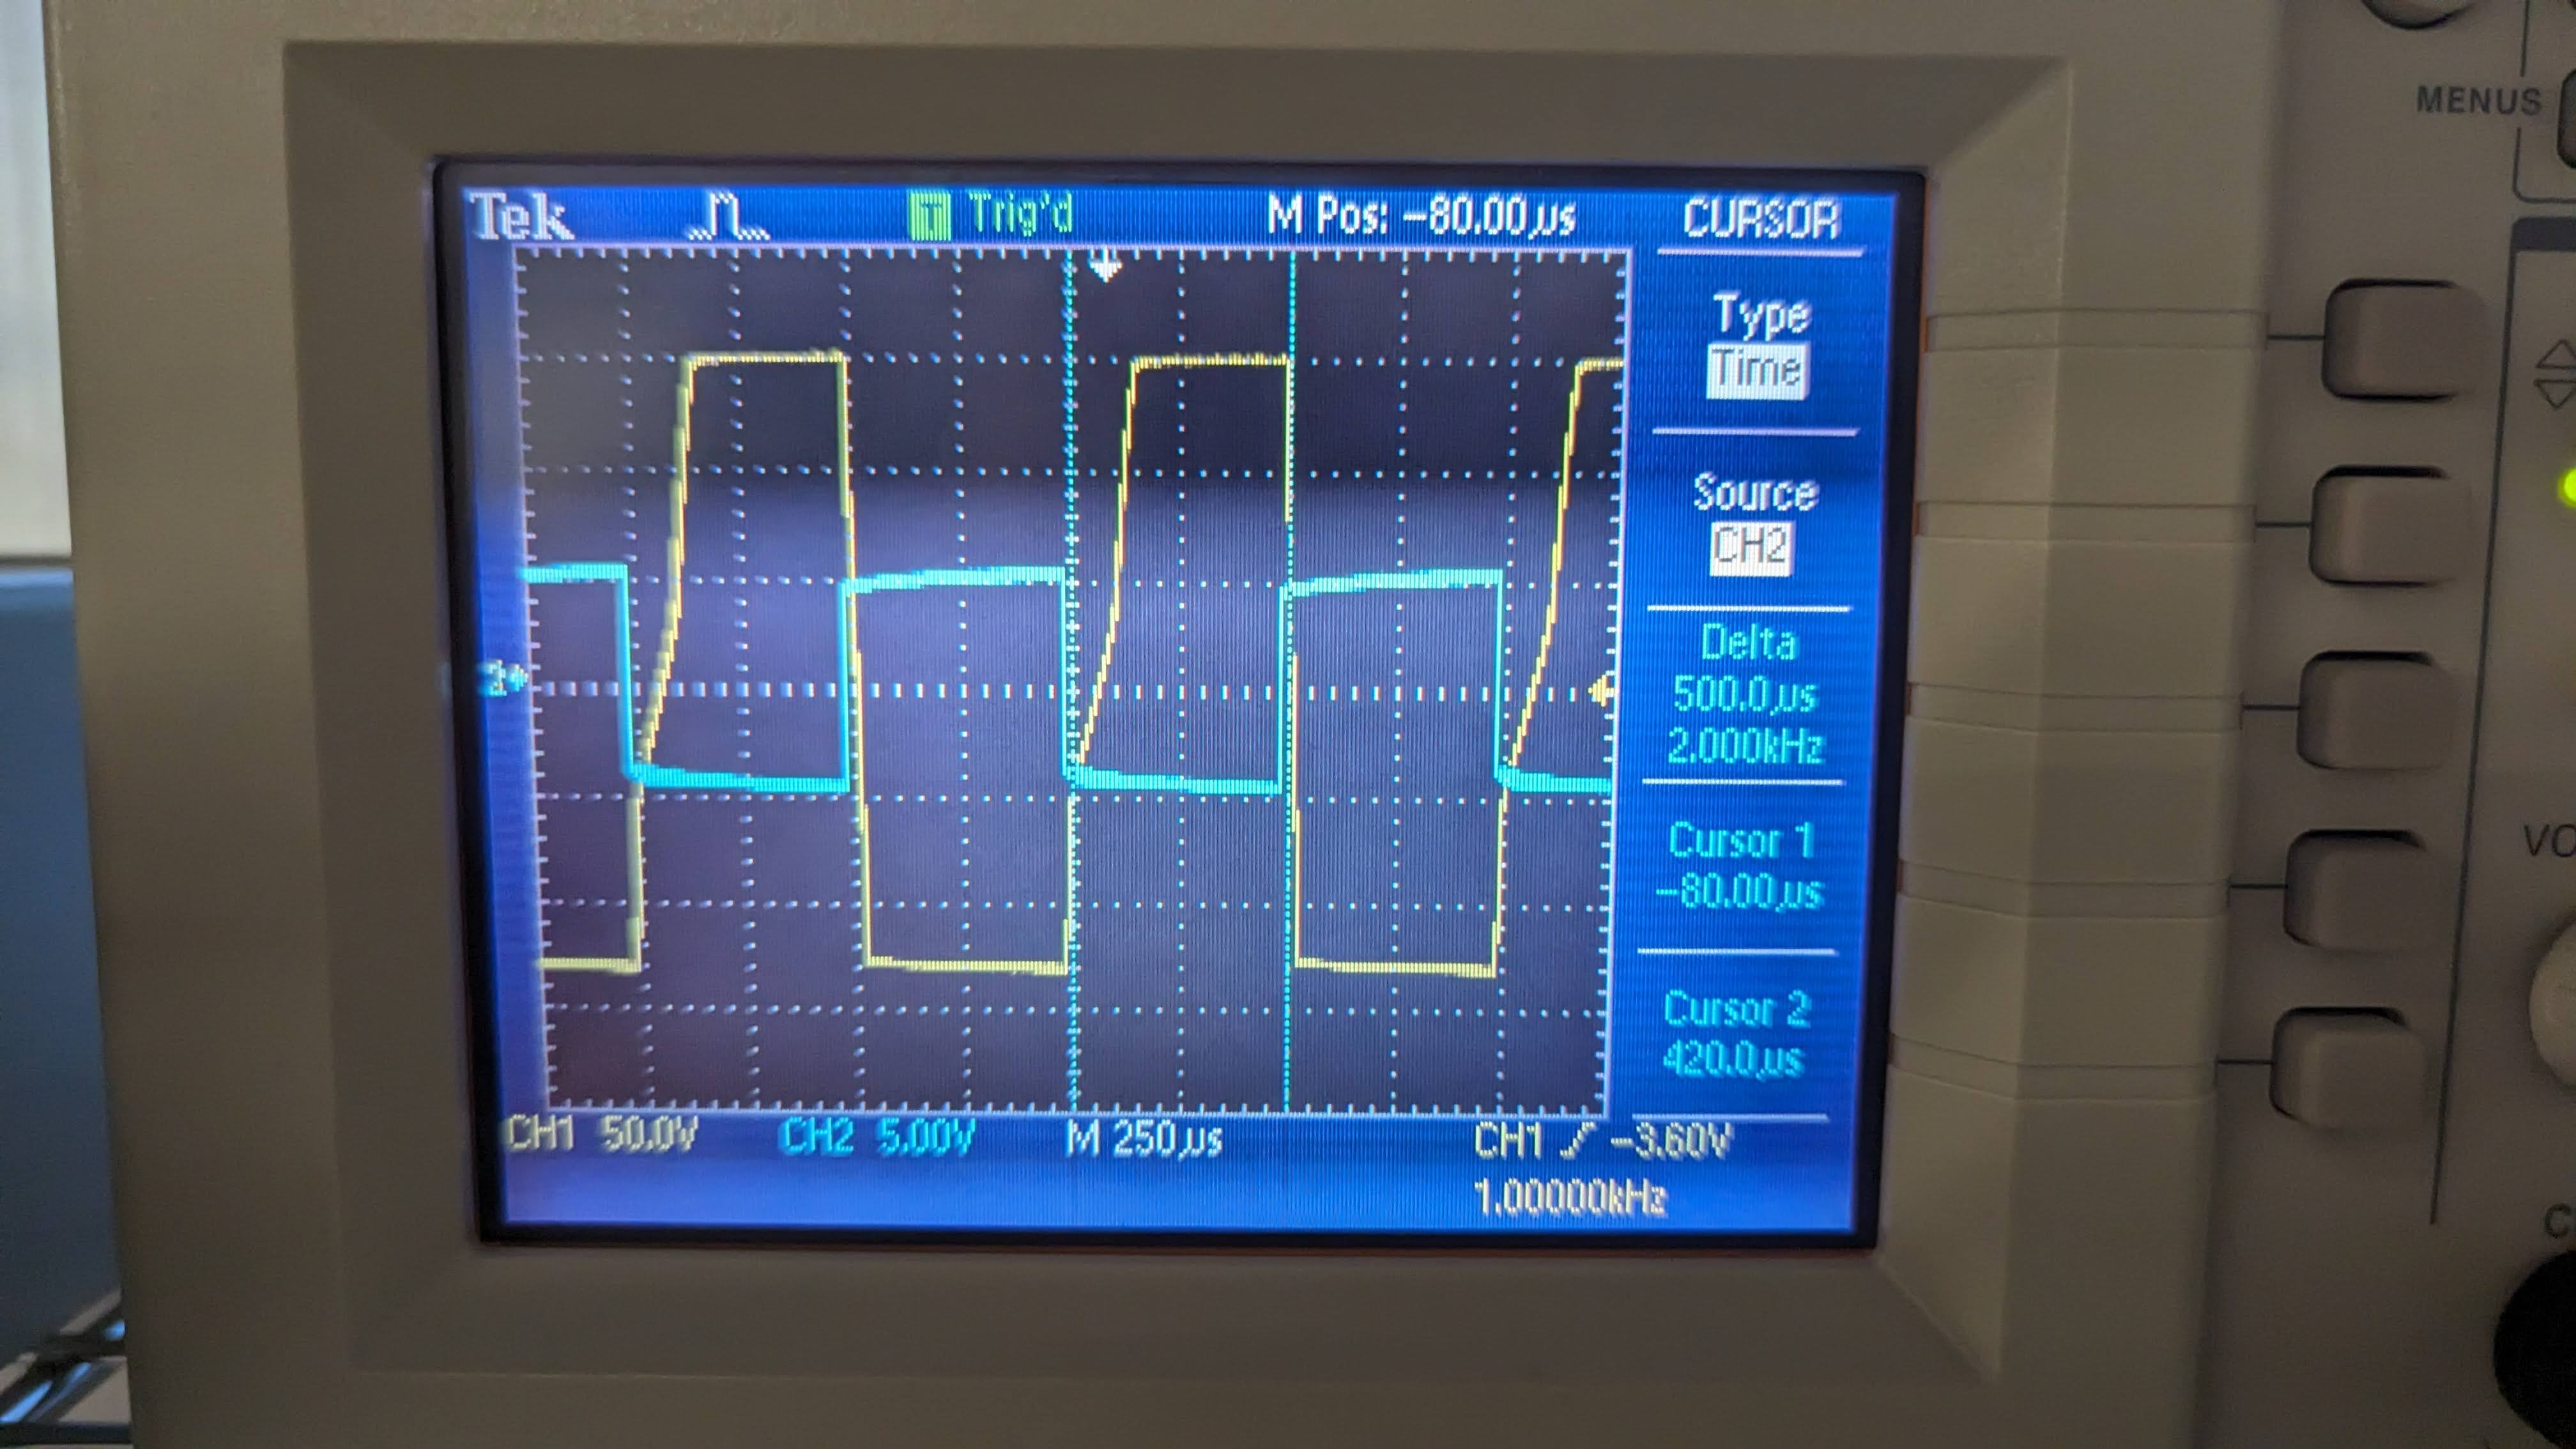
\includegraphics[width=0.8\textwidth]{2-4}
    \caption{Plot for question 2.2 of the monostable multivibrator when the frequency is increased to 1kHz. The output voltage pulse (blue) is ``squished'' between the input square wave form (yellow).}
    \label{fig:2-4}
\end{figure}

\end{document}
